\documentclass{article} % For LaTeX2e
\usepackage{nips12submit_e,times}
%\documentstyle[nips12submit_09,times,art10]{article} % For LaTeX 2.09

\usepackage[latin1]{inputenc}
% \usepackage[francais]{babel}
\usepackage[T1]{fontenc}
% For figures
\usepackage{graphicx} % more modern
%\usepackage{epsfig} % less modern
\usepackage{subfigure}
%\usepackage{mathtools}

\usepackage[ruled,algo2e]{algorithm2e}
\usepackage{hyperref}


\usepackage{amsmath}
\usepackage{amsthm}
\usepackage{amssymb}
\usepackage{amscd}

\usepackage{mathtools}
\mathtoolsset{showonlyrefs=true}

\newcommand{\argmax}{\operatorname*{argmax}} %\operatorname* pour les op. pouvant admettre des limites...
\newcommand{\argmin}{\operatorname*{argmin}}
\newcommand{\diag}{\operatorname*{diag}}

\newcommand{\p}{\mathcal{P}}
\newcommand{\R}{\mathcal{R}}
\newcommand{\s}{\mathcal{S}}
\newcommand{\A}{\mathcal{A}}
\newcommand{\X}{\mathcal{X}}
\newcommand{\Y}{\mathcal{Y}}
\newcommand{\D}{\mathcal{D}}
\newcommand{\T}{\mathcal{T}}
\newcommand{\lc}{\mathcal{L}}
\newcommand{\E}{\mathbb{E}}
\newcommand{\prob}{\mathbb{P}}
\newcommand{\Mu}{\boldsymbol{\mu}}
%\newcommand{\Xi}{\boldsymbol{\xi}}


\newtheorem{theorem}{Theorem}
\newtheorem{prop}[theorem]{Proposition}

\title{Inverse Reinforcement Learning \\ through Structured Classification}

\author{
Edouard Klein$^{1,2}$\\
$^{1}$LORIA -- team ABC\\
Nancy, France\\
\texttt{edouard.klein@supelec.fr} \And
Matthieu Geist$^{2}$\\
$^{2}$Sup�lec -- IMS-MaLIS Research Group\\
Metz, France\\
\texttt{matthieu.geist@supelec.fr}
\And Bilal Piot$^{2,3}$, Olivier Pietquin$^{2,3}$\\
$^{3}$ UMI 2958 (GeorgiaTech-CNRS)\\
Metz, France\\
\texttt{$\{$bilal.piot,olivier.pietquin$\}$@supelec.fr} }


\newcommand{\fix}{\marginpar{FIX}}
\newcommand{\new}{\marginpar{NEW}}

\nipsfinalcopy % Uncomment for camera-ready version

\begin{document}


\maketitle


\begin{abstract}
  This paper adresses the inverse reinforcement learning (IRL) problem, that
  is inferring a reward for which a demonstrated expert behavior is
  optimal. We introduce a new algorithm, SCIRL, whose principle is to use
  the so-called feature expectation of the expert as the
  parameterization of the score function of a multi-class
  classifier. This approach produces a reward function for which the
  expert policy is provably near-optimal. Contrary to most of
  existing IRL algorithms, SCIRL does not require solving the
  direct RL problem. Moreover, with an appropriate heuristic, it can succeed with only trajectories sampled
  according to the expert behavior. This is illustrated on a car
  driving simulator.
\end{abstract}



\section{Introduction}
\label{sec:intro}

Inverse reinforcement learning (IRL)~\cite{Russell:1998} consists in
finding a reward function such that a demonstrated expert behavior
is optimal. Many IRL algorithms (to be briefly reviewed in
Sec.~\ref{sec:relatedWorks}) search for a reward function such that
the associated optimal policy induces a distribution over
trajectories (or some measure of this distribution) which matches
the one induced by the expert. Often, this distribution is
characterized by the so-called feature expectation (see
Sec.~\ref{subsec:background:irl}): given a reward function linearly
parameterized by some feature vector, it is the expected discounted
cumulative feature vector for starting in a given state, applying a
given action and following the related policy.

In this paper, we take a  different route. The expert behavior could
be mimicked by a supervised learning algorithm generalizing the
mapping from states to actions. Here, we consider generally
multi-class classifiers which compute from a training set the
parameters of a linearly parameterized score function; the decision
rule for a given state is the argument (the action) which maximizes
the score function for this state (see
Sec.~\ref{subsec:background:classif}). The basic idea of our SCIRL
(Structured Classification-based IRL) algorithm is simply to take an
estimate of the expert feature expectation as the parameterization
of the score function (see Sec.~\ref{subsec:scirl:algo}). The
computed parameter vector actually defines a reward function for
which we show the expert policy to be near-optimal
(Sec.~\ref{subsec:scirl:analysis}).

Contrary to most existing IRL algorithms, a clear advantage of SCIRL
is that it does not require solving repeatedly the direct
reinforcement learning (RL) problem. It requires estimating the
expert feature expectation, but this is roughly a policy evaluation
problem (for an observed policy, so is less involved than repeated
policy optimization problems), see Sec.~\ref{sec:practicalApproach}.
Moreover, up to the use of some heuristic, SCIRL may be trained
solely from transitions sampled from the expert policy (no need to
sample the whole dynamic). We illustrate this on a car driving
simulator in Sec.~\ref{sec:experiments}.


\section{Background and Notations}
\label{sec:background}

\subsection{(Inverse) Reinforcement Learning}
\label{subsec:background:irl}

A Markov Decision process (MDP)~\cite{Puterman:1994} is a tuple
$\{\s,\A,\p,\R,\gamma\}$ where $\s$ is the finite state
space\footnote{This work can be extended to compact state spaces, up
to some technical aspects.}, $\A$ the finite actions space, $\p =
\{P_a = (p(s'|s,a))_{1\leq s,s'\leq |\s|}, a\in\A\}$ the set of
Markovian transition probabilities, $\R\in\mathbb{R}^\s$ the
state-dependent reward function and $\gamma$ the discount factor. A
deterministic policy $\pi\in\s^\A$ defines the behavior of an agent.
The quality of this control is quantified by the value function
$v_\R^\pi\in\mathbb{R}^\s$, associating to each state the cumulative
discounted reward for starting in this state and following the
policy $\pi$ afterwards: $v_\R^\pi(s) = \E[\sum_{t\geq 0} \gamma^t
\R(S_t)|S_0=s,\pi]$. An optimal policy $\pi_\R^*$ (according to the
reward function $\R$) is a policy of associated value function
$v^*_\R$ satisfying $v_\R^* \geq v_\R^\pi$, for any policy $\pi$ and
componentwise.

Let $P_\pi$ be the stochastic matrix $P_\pi =
(p(s'|s,\pi(s)))_{1\leq s,s'\leq |\s|}$. With a slight abuse of
notation, we may write $a$ the policy which associates the action
$a$ to each state $s$. The Bellman evaluation (resp. optimality)
operators $T^\pi_\R\text{ (resp. $T^*_\R$)}:\mathbb{R}^\s
\rightarrow \mathbb{R}^\s$ are defined as $T^\pi_\R v = \R + \gamma
P_\pi v$ and $T_\R^*v = \max_\pi T_\R^\pi v$.
%\begin{equation}
%  T^\pi_\R v = \R + \gamma P_\pi v \text{ and } T_\R^*v = \max_\pi T_\R^\pi v.
%\end{equation}
These operators are contractions and $v_\R^\pi$ and $v^*_\R$ are
their respective fixed-points: $v_\R^\pi = T^\pi_\R v_\R^\pi$ and
$v^*_\R = T^*_\R v^*_\R$. The action-value function
$Q^\pi\in\mathbb{R}^{\s\times \A}$ adds a degree of freedom on the
choice of the first action, it is formally defined as $Q_\R^\pi(s,a)
= [T^a_\R v^\pi_\R](s)$. We also write $\rho_\pi$ the stationary
distribution of the policy $\pi$ (satisfying $\rho_\pi^\top P_\pi =
\rho_\pi^\top$).

Reinforcement learning and approximate dynamic programming aim at
estimating the optimal control policy $\pi^*_\R$ when the model
(transition probabilities and the reward function) is unknown (but
observed through interactions with the system to be controlled) and
when the state space is too large to allow exact representations of
the objects of interest (as value functions or
policies)~\cite{Bertsekas:1996,Sutton:1998,szepesvari2010c}.
%
We refer to this as the direct problem.
%
On the contrary, (approximate) inverse reinforcement
learning~\cite{Ng:2000} aim at estimating a reward function for
which an observed policy is (nearly) optimal.
%
Let us call this policy the expert policy, denoted $\pi_E$. We may
assume that it optimizes some unknown reward function $\R_E$. The
aim of IRL is to compute some reward $\hat{\R}$ such that the expert
policy is (close to be) optimal, that is such that $v^*_{\hat{\R}}
\approx v^{\pi_E}_{\hat{\R}}$.
%
We refer to this as the inverse problem.

Similarly to the direct problem, the state space may be too large
for the reward function to admit a practical exact representation.
Therefore, we restrict our search of a good reward among linearly
parameterized functions. Let $\phi(s) = (\phi_1(s)  \dots
\phi_p(s))^\top$
%\begin{pmatrix}
%  \phi_1(s) & \dots & \phi_p(s)
%\end{pmatrix}^\top$
be a feature vector composed of $p$ basis function
$\phi_i\in\mathbb{R}^\s$, we define the  parameterized reward
functions as $\R_\theta(s) = \theta^\top \phi(s) = \sum_{i=1}^p
\theta_i \phi_i(s)$.
%\begin{equation}
%  \R_\theta(s) = \theta^\top \phi(s) = \sum_{i=1}^p \theta_i \phi_i(s).
%\end{equation}
Searching a good reward thus reduces to searching a good parameter
vector $\theta \in\mathbb{R}^p$. Notice that we will use
interchangeably $\R_\theta$ and $\theta$ as subscripts
(\textit{e.g.}, $v_\theta^\pi$ for $v_{\R_\theta}^\pi$).
Parameterizing the reward this way implies a related
parameterization for the action-value function:
\begin{equation}
  Q^\pi_\theta(s,a) = \theta^\top \mu^\pi(s,a) \text{ with }
  \mu^\pi(s,a) = \E[\sum_{t\geq 0} \gamma^t
  \phi(S_t)|S_0=s,A_0=a,\pi].
  \label{eq:def:mu}
\end{equation}
Therefore, the action-value function shares the parameter vector of
the reward function, with an associated feature vector $\mu^\pi$
called the \emph{feature expectation}. This notion will be of
primary importance for the contribution of this paper. Notice that
each component $\mu_i^\pi$ of this feature vector is actually the
action-value function of the policy $\pi$ assuming the reward is
$\phi_i$: $\mu_i^\pi(s,a) = Q^\pi_{\phi_i}(s,a)$. Therefore, any
algorithm designed for estimating an action-value function may be
used to estimate the feature expectation, such as Monte-Carlo
rollouts or temporal difference learning~\cite{Klein:2011}.



\subsection{Classification with Linearly Parameterized Score
Functions} \label{subsec:background:classif}

Let $\X$ be a compact or a finite set (of inputs to be classified)
and let $\Y$ be a finite set (of labels). Assume that inputs $x\in
\X$  are drawn according to some unknown distribution $\prob(x)$ and
that there exists some oracle which associates to each of these
inputs a label $y\in Y$ drawn according to the unknown conditional
distribution $\prob(y|x)$. Generally speaking, the goal of
multi-class classification is, given a training set
$\{(x_i,y_i)_{1\leq i \leq N}\}$ drawn according to $\prob(x,y)$, to
produce a decision rule $g\in\Y^\X$ which aims at minimizing the
classification error $\E[\chi_{\{g(x)\neq y\}}] = \prob(g(x)\neq
y)$, where $\chi$ denotes the indicator function.

Here, we consider a more restrictive set of classification
algorithms. We assume that the decision rule associates to an input
the argument which maximizes a related score function, this score
function being linearly parameterized and the associated parameters
being learnt by the algorithm. More formally, let $\psi(s,a) =
(\psi_1(x,y)  \dots  \psi_d(x,y))^\top\in \mathbb{R}^d$
%\begin{pmatrix}   \psi_1(x,y) & \dots & \psi_d(x,y)
%\end{pmatrix}^\top \in \mathbb{R}^d$
be a feature vector whose components are $d$ basis functions
$\psi_i\in\mathbb{R}^{\X\times\Y}$. The linearly parameterized score
function $s_w\in\mathbb{R}^{\X\times \Y}$ of parameter vector
$w\in\mathbb{R}^d$ is defined as $s_w(x,y) = w^\top \psi(x,y)$. The
associated decision rule $g_w\in{\Y^\X}$ is defined as $g_w(x) \in
\argmax_{y\in\Y}s_w(x,y)$. Using a training set $\{(x_i,y_i)_{1\leq
i\leq N}\}$, a linearly parameterized score function-based
multi-class classification (MC$^2$ for short) algorithm computes a
parameter vector $\theta_c$. The quality of the solution is
quantified by the classification error $\epsilon_c =
\prob(g_{\theta_c}(x)\neq y)$.

We do not consider a specific MC$^2$ algorithm, as long as it
classifies inputs by maximizing the argument of a linearly
parameterized score function. For example, one may choose a
multi-class support vector machine~\cite{Guermeur:2007} (taking the
kernel induced by the feature vector) or a structured large margin
approach~\cite{Taskar:2005}. Other choices may be possible, one can
choose its preferred algorithm.



\section{Structured Classification for Inverse Reinforcement
Learning} \label{sec:scirl}

\subsection{General Algorithm}
\label{subsec:scirl:algo}

Consider the classification framework of
Sec.~\ref{subsec:background:classif}. The input $x$ may be seen as a
state and the label $y$ as an action. Then, the decision rule
$g_w(x)$ can be interpreted as a policy which is greedy according to
the score function $w^\top \psi(x,y)$, which may itself be seen as
an action-value function. Making the parallel with
Eq.~\eqref{eq:def:mu}, if $\psi(x,y)$ is the feature expectation of
some policy $\pi$ which produces labels of the training set, and if
the classification error is small, then $w$ will be the parameter
vector of a reward function for which we may hope the policy $\pi$
to be near optimal. Based on these remarks, we're ready to present
the proposed Structured Classification-based IRL (SCIRL) algorithm.

Let $\pi_E$ be the expert policy from which we would like to recover
a reward function. Assume that we have a training set $\D =
\{(s_i,a_i=\pi_E(s_i))_{1\leq i\leq N}\}$ where states are sampled
according to the expert stationary distribution\footnote{For
example, if the Markov chain induced by the expert policy is
fast-mixing, sampling a trajectory will quickly lead to sample
states according to this distribution.} $\rho_E = \rho_{\pi_E}$.
Assume also that we have an estimate $\hat{\mu}^{\pi_E}$ of the
expert feature expectation $\mu^{\pi_E}$ defined in
Eq.~\eqref{eq:def:mu}. How to practically estimate this quantity is
postponed to Sec.~\ref{subsec:practicalApproach:muE}; however,
recall that estimating $\mu^{\pi_E}$ is simply a \emph{policy
evaluation} problem (estimating the action-value function of a given
policy), as noted in Sec.~\ref{subsec:background:irl}. Assume also
that an MC$^2$ algorithm has been chosen. The proposed algorithm
simply consists in choosing $\theta^\top\hat{\mu}^{\pi_E}(s,a)$ as
the linearly parameterized score function, training the classifier
on $\D$ which produces a parameter vector $\theta_c$, and outputting
the reward function $\R_{\theta_c}(s) = \theta_c^\top \phi(s)$.

\begin{algorithm2e}%[tbh]
    %\small
  \SetAlgoVlined
  \caption{SCIRL algorithm}
  \label{algo:scirl}
  %
  \BlankLine
  \emph{\textbf{Given}} a training set $\D = \{(s_i,a_i=\pi_E(s_i))_{1\leq i\leq N}\}$,
  an estimate $\hat{\mu}^{\pi_E}$ of the expert feature expectation $\mu^{\pi_E}$ and an MC$^2$ algorithm\;
  %
  \BlankLine
  \emph{\textbf{Compute}} the parameter vector $\theta_c$ using the
  MC$^2$ algorithm
  fed with the training set $\D$ and considering the parameterized score function
  $\theta^\top\hat{\mu}^{\pi_E}(s,a)$\;
  %
  \BlankLine
  \emph{\textbf{Output}} the reward function $\R_{\theta_c}(s) = \theta_c^\top\phi(s)$ \;
\end{algorithm2e}

The proposed approach is summarized in Alg.~\ref{algo:scirl}. We
call this Structured Classification-based IRL because using the
(estimated) expert feature expectation as the feature vector for the
classifier somehow implies taking into account the MDP structure
into the classification problem and allows outputting a reward
vector. Notice that contrary to most of existing IRL
%and apprenticeship learning
algorithms, SCIRL does not require solving the direct problem. If it
possibly requires estimating the expert feature expectation, it is
just a policy evaluation problem, less difficult than the policy
optimization issue involved by the direct problem. This is further
discussed in Sec.~\ref{sec:relatedWorks}.
%
%Now, we formally show that the proposed approach makes sens, as long
%as $\mu^{\pi_E}$ is well estimated and as long as the classification
%error is small.


\subsection{Analysis}
\label{subsec:scirl:analysis}

In this section, we show that the expert policy $\pi_E$ is close to
be optimal according to the reward function $\R_{\theta_c}$, more
precisely that
$\E_{s\sim\rho_E}[v^*_{\theta_c}(s)-v^{\pi_E}_{\theta_c}(s)]$ is
small. Before stating our main result, we need to introduce some
notations and to define some objects.

We will use the first order discounted future state distribution
concentration coefficient $C_f$~\cite{Munos:2007}:
\begin{equation}
  C_f = (1-\gamma)\sum_{t\geq 0} \gamma^t c(t) \text{ with } c(t) =
  \max_{\pi_1,\dots,\pi_t,s\in\s}\frac{(\rho_E^\top P_{\pi_1}\dots
  P_{\pi_t})(s)}{\rho_E(s)}.
\end{equation}
We note $\pi_c$ the decision rule of the classifier: $\pi_c(s) \in
\argmax_{a\in \A} \theta_c^\top\hat{\mu}^{\pi_E}(s,a)$. The
classification error is therefore $\epsilon_c =
\E_{s\sim\rho_E}[\chi_{\{\pi_c(s)\neq\pi_E(s)\}}] \in [0,1]$. We
write $\hat{Q}^{\pi_E}_{\theta_c} = \theta_c^\top \hat{\mu}^{\pi_E}$
the score function computed from the training set $\D$ (which can be
interpreted as an approximate action-value function). Let also
$\epsilon_{\mu} = \hat{\mu}^{\pi_E} - \mu^{\pi_E}:\s\times\A
\rightarrow  \mathbb{R}^p$ be the feature expectation error.
Consequently, we define the action-value function error as
$\epsilon_Q = \hat{Q}^{\pi_E}_{\theta_c} - Q^{\pi_E}_{\theta_c} =
\theta_c^\top(\hat{\mu}^{\pi_E} - \mu^{\pi_E}) = \theta_c^\top
\epsilon_\mu:\s\times\A\rightarrow\mathbb{R}$. We finally define the
mean delta-max action-value function error as $\bar{\epsilon}_Q =
\E_{s\sim\rho_E}[\max_{a\in\A}\epsilon_Q(s,a) -
\min_{a\in\A}\epsilon_Q(s,a)]\geq 0$.



\begin{theorem}
  \label{th}
  Let $\R_{\theta_c}$ be the reward function outputted by
  Alg.~\ref{algo:scirl}. Let also the quantities $C_f$, $\epsilon_c$
  and $\bar{\epsilon}_Q$ be defined as above. We have
  %
%  the concentration coefficient $C_f$,
%  the classification error $\epsilon_c$ and the mean-max
%  action-value function error $\bar{\epsilon}_Q$ be defined as
%  above. Then, we have
  \begin{equation}
    0\leq
    \E_{s\sim\rho_E}[v^*_{\R_{\theta_c}}-v^{\pi_E}_{\R_{\theta_c}}]
    \leq \frac{C_f}{1-\gamma}\left(\bar{\epsilon}_Q +
    \epsilon_c\frac{2\gamma\|\R_{\theta_c}\|_\infty}{1-\gamma}
%    \epsilon_c\frac{2\gamma}{1-\gamma}\min(\|\R_{\theta_c}\|_\infty,
%    C_p \E_{s\sim\rho_E}[\R_{\theta_c}(s)])
    \right).
  \end{equation}
\end{theorem}
\begin{proof}
  As the proof only relies on the reward $\R_{\theta_c}$, we
  omit the related subscripts to keep the notations simple
  (\textit{e.g.}, $v^\pi$ for
  $v^\pi_{\theta_c}=v^\pi_{\R_{\theta_c}}$ or $\R$ for $\R_{\theta_c}$). First, we link
  the error $\E_{s\sim\rho_E}[v^*(s)-v^{\pi_E}(s)]$ to the
  Bellman residual $\E_{s\sim\rho_E}[[T^*v^{\pi_E}](s)-v^{\pi_E}(s)]$.
  %
  % A second step consists in bounding this residual.
  %
  Componentwise, we have that:
  \begin{align}
    v^* - v^{\pi_E} &= T^* v^*  - T^{\pi^*}v^{\pi_E} +
    T^{\pi^*}v^{\pi_E} - T^* v^{\pi_E} + T^* v^{\pi_E} - v^{\pi_E}
    \\
    &\stackrel{(a)}{\leq} \gamma P_{\pi^*}(v^*-v^{\pi_E}) + T^*
    v^{\pi_E} - v^{\pi_E}
    %
    \stackrel{(b)}{\leq} (I-\gamma
    P_{\pi^*})^{-1} (T^* v^{\pi_E} - v^{\pi_E}).
  \end{align}
  Inequality $(a)$ holds because $T^{\pi^*} v^{\pi_E}\leq T^*
  v^{\pi_E}$ and inequality $(b)$ holds thanks
  to~\cite[Lemma~4.2]{Munos:2007}. Moreover, $v^*$ being optimal we
  have that $v^*-v^{\pi_E}\geq 0$ and $T^*$ being the Bellman
  optimality operator, we have $T^* v^{\pi_E}\geq
  T^{\pi_E}v^{\pi_E}=v^{\pi_E}$. Additionally, remark that
  $(I-\gamma P_{\pi^*})^{-1} = \sum_{t\geq 0}\gamma^t P_{\pi^*}^t$.
  Therefore, using the definition of the concentration coefficient
  $C_f$, we have that:
  \begin{equation}
    0\leq\E_{s\sim\rho_E}[v^*(s)-v^{\pi_E}(s)] \leq \frac{C_f}{1-\gamma}
    \E_{s\sim\rho_E}\left[[T^*v^{\pi_E}](s) - v^{\pi_E}(s)\right].
    \label{eq:proof:residual}
  \end{equation}
  This results actually follows closely the one
  of~\cite[Theorem~4.2]{Munos:2007}. There remains to bound the
  Bellman residual $\E_{s\sim\rho_E}[[T^*v^{\pi_E}](s) -
  v^{\pi_E}(s)]$. Considering the following decomposition,
  \begin{equation}
    T^* v^{\pi_E} - v^{\pi_E} = T^* v^{\pi_E} - T^{\pi_c}v^{\pi_E}
    + T^{\pi_c}v^{\pi_E}- v^{\pi_E},
    \label{eq:proof:decomposition}
  \end{equation}
  we will bound $\E_{s\sim\rho_E}[[T^* v^{\pi_E}](s) - [T^{\pi_c}v^{\pi_E}](s)]$
  and $\E_{s\sim\rho_E}[[T^{\pi_c}v^{\pi_E}](s) - v^{\pi_E}(s)]$.

  The policy $\pi_c$ (the decision rule of the classifier) is greedy
  with respect to
  $\hat{Q}^{\pi_E}=\theta_c^\top\hat{\mu}^{\pi_E}$. Therefore, for any state-action couple
  $(s,a)\in\s\times \A$ we have:
  \begin{equation}
    \hat{Q}^{\pi_E}(s,\pi_c(s))\geq
    \hat{Q}^{\pi_E}(s,a)
    \Leftrightarrow
    Q^{\pi_E}(s,a) \leq Q^{\pi_E}(s,\pi_c(s)) +
    \epsilon_Q(s,\pi_c(s)) - \epsilon_Q(s,a).
  \end{equation}
  By definition, $Q^{\pi_E}(s,a) = [T^a v^{\pi_E}](s)$ and
  $Q^{\pi_E}(s,\pi_c(s)) = [T^{\pi_c} v^{\pi_E}](s)$. Therefore, for $s\in\s$:
  \begin{align}
    \forall a\in A,\; [T^a v^{\pi_E}](s) &\leq [T^{\pi_c}
    v^{\pi_E}](s) + \epsilon_Q(s,\pi_c(s))-\epsilon_Q(s,a)
    \\
    \Rightarrow [T^* v^{\pi_E}](s) &\leq [T^{\pi_c}
    v^{\pi_E}](s) + \max_{a\in \A}\epsilon_Q(s,a)-\min_{a\in
    \A}\epsilon_Q(s,a).
  \end{align}
  Taking the expectation according to $\rho_E$ and noticing that
  $T^* v^{\pi_E}\geq v^{\pi_E}$, we bound the first
  term:
  \begin{equation}
    0 \leq \E_{s\sim\rho_E}\left[ [T^* v^{\pi_E}](s) - [T^{\pi_c}
    v^{\pi_E}](s)\right] \leq \bar{\epsilon}_Q.
    \label{eq:proof:b1}
  \end{equation}
  There finally remains to bound the term $\E_{s\sim\rho_E}[[T^{\pi_c}v^{\pi_E}](s) -
  v^{\pi_E}(s)]$.

  Let us write $M\in\mathbb{R}^{|\s|\times |\s|}$ the diagonal matrix
  defined as $M = \diag (\chi_{\{\pi_c(s)\neq\pi_E(s)\}})$. Using
  this, the Bellman operator $T^{\pi_c}$ may be written as, for any $v\in\mathbb{R}^\s$:
  \begin{equation}
    T^{\pi_c}v = \R + \gamma M P_{\pi_c} v + \gamma (I-M)P_{\pi_E} v
    = \R + \gamma P_{\pi_E} v + \gamma M (P_{\pi_c}-P_{\pi_E})v.
  \end{equation}
  Applying this operator to $v^{\pi_E}$ and recalling that $\R +
  \gamma P_{\pi_E} v^{\pi_E} = T^{\pi_E} v^{\pi_E} = v^{\pi_E}$, we
  get:
  \begin{equation}
    T^{\pi_c}v^{\pi_E} - v^{\pi_E} = \gamma M
    (P_{\pi_c}-P_{\pi_E})v^{\pi_E}
    \Rightarrow |\rho_E^\top (T^{\pi_c}v^{\pi_E} - v^{\pi_E})| = \gamma
    |\rho_E^\top M (P_{\pi_c}-P_{\pi_E})v^{\pi_E}|.
  \end{equation}
  One can easily see that $\|(P_{\pi_c}-P_{\pi_E})v^{\pi_E}\|_\infty
  \leq \frac{2}{1-\gamma}\|\R\|_\infty$, which allows bounding the
  last term:
  \begin{equation}
    |\E_{s\sim\rho_E}[[T^{\pi_c}v^{\pi_E}](s) - v^{\pi_E}(s)]| \leq
    \epsilon_c \frac{2\gamma}{1-\gamma} \|\R\|_\infty.
    \label{eq:proof:b2}
  \end{equation}
  Injecting bounds of Eqs.~\eqref{eq:proof:b1}
  and~\eqref{eq:proof:b2} into Eq.~\eqref{eq:proof:residual} gives the
  stated result.%, which concludes the proof.
%  Injecting bounds of Eqs.~\eqref{eq:proof:b1}
%  and~\eqref{eq:proof:b2} into Eq.~\eqref{eq:proof:residual} using the
%  decomposition of Eq.~\eqref{eq:proof:decomposition} gives the
%  stated result:
%  \begin{equation}
%    0\leq\E_{s\sim\rho_E}[v^*(s)-v^{\pi_E}(s)] \leq
%    \frac{C_f}{1-\gamma} \left(\bar{\epsilon}_Q + \epsilon_c \frac{2\gamma}{1-\gamma} \|\R\|_\infty
%    \right).
%  \end{equation}
%  This concludes the proof.
\end{proof}

This result shows that if the expert feature expectation is well
estimated (in the sense that the estimation error $\epsilon_\mu$ is
small for states sampled according to the expert stationary policy
and for all actions) and if the classification error $\epsilon_c$ is
small, then the proposed generic algorithm outputs a reward function
$\R_{\theta_c}$ for which the expert policy will be near optimal. A
direct corollary of Th.~\ref{th} is that given the true expert
feature expectation $\mu^{\pi_E}$ and a perfect classifier
($\epsilon_c=0$), $\pi_E$ is the unique optimal policy for
$\R_{\theta_c}$.

One may argue that this bounds trivially holds for the null reward
function (a reward often exhibited to show that IRL is an ill-posed
problem), obtained if $\theta_c=0$. However, recall that the
parameter vector $\theta_c$ is computed by the classifier. With
$\theta_c=0$, the decision rule would be a random policy and we
would have $\epsilon_c = \frac{|\A|-1}{|\A|}$, the worst possible
classification error. This case is really unlikely. Therefore, we
advocate that the proposed approach somehow allows disambiguating
the IRL problem (at least, it does not output trivial reward
functions such as the null vector).
%
Also, this bound is scale-invariant: one could impose
$\|\theta_c\|=1$ or normalize (action-) value functions by
$\|\R_{\theta_c}\|_\infty^{-1}$.

One should notice that there is a hidden dependency of the
classification error $\epsilon_c$ to the estimated expert feature
expectation $\hat{\mu}^{\pi_E}$. Indeed, the minimum classification
error depends on the hypothesis space spanned by the chosen score
function basis functions for the MC$^2$ algorithm (here
$\hat{\mu}^{\pi_E}$). Nevertheless, provided a good representation
for the reward function (that is a good choice of basis functions
$\phi_i$) and a small estimation error, this should not be a
practical problem.

Finally, if our bound relies on the generalization errors
$\epsilon_c$ and $\bar{\epsilon}_Q$, the classifier will only use
$(\hat{\mu}^{\pi_E}(s_i,a))_{1\leq i\leq N,a\in\A}$ in the training
phase, where $s_i$ are the states from the set $\D$. It outputs
$\theta_c$, seen as a reward function, thus the estimated feature
expectation $\hat{\mu}^{\pi_E}$ is no longer required. Therefore,
practically it should be sufficient to estimate well
$\hat{\mu}^{\pi_E}$ on state-action couples $(s_i,a)_{1\leq i\leq
N,a\in\A}$, which allows envisioning Monte-Carlo rollouts for
example.

\section{A Practical Approach}
\label{sec:practicalApproach}

\subsection{Estimating the Expert Feature Expectation}
\label{subsec:practicalApproach:muE}

SCIRL relies on an estimate $\hat{\mu}^{\pi_E}$ of the expert
feature expectation. Basically, this is a policy evaluation problem.
An already made key observation is that each component of
$\mu^{\pi_E}$ is the action-value function of $\pi_E$ for a reward
function $\phi_i$: $\mu_i^{\pi_E}(s,a) = Q^{\pi_E}_{\phi_i}(s,a) =
[T^a_{\phi_i} v^{\pi_E}_{\phi_i}](s)$. We briefly review its exact
computation and possible estimation approaches, and consider
possible heuristics.
%possibly considering some heuristics.

If the model is known, the feature expectation can be computed
explicitly. Let $\Phi\in\mathbb{R}^{|\s|\times p}$ be the feature
matrix whose rows contain the feature vectors $\phi(s)^\top$ for all
$s\in\s$.
%
%(equivalently, whose columns contain the basis functions $\phi_i$
%for $1\leq i\leq p$).
%
For a fixed $a\in A$, let $\Mu^{\pi_E}_a \in\mathbb{R}^{|\s|\times
p}$ be the feature expectation matrix whose rows are the expert
feature vectors, that is $(\mu^{\pi_E}(s,a))^\top$ for any $s\in\s$.
With these notations, we have $\Mu_a^{\pi_E} = \Phi + \gamma
P_a(I-\gamma P_{\pi_E})^{-1} \Phi$.
%\begin{equation}
%  \forall a\in\A,\; \Mu_a^{\pi_E} = \Phi + \gamma P_a(I-\gamma
%  P_{\pi_E})^{-1} \Phi.
%\end{equation}
%Therefore, knowing the model (the dynamic), the expert feature
%expectation can be easily computed.
Moreover, the related computational cost is the same order of
magnitude as evaluating a single policy (as the costly part,
computing $(I-\gamma P_{\pi_E})^{-1}$, is shared by all components).

If the model is unknown, any temporal difference learning algorithm
can be used to estimate the expert feature
expectation~\cite{Klein:2011}, as LSTD (Least-Squares Temporal
Differences)~\cite{Bradtke:1996}. Let $\psi:\s\times \A \rightarrow
\mathbb{R}^d$ be a feature vector composed of $d$ basis functions
$\psi_i \in\mathbb{R}^{\s\times \A}$. Each component $\mu_i^{\pi_E}$
of the expert feature expectation is parameterized by a vector
$\xi_i\in\mathbb{R}^d$: $\mu_i^{\pi_E}(s,a)\approx \xi_i^\top
\psi(s,a)$. Assume that we have a training set
$\{(s_i,a_i,s'_i,a'_i=\pi_E(s'_i))_{1\leq i \leq M}\}$ with actions
$a_i$ not necessarily sampled according to policy $\pi_E$
(\textit{e.g.}, this may be obtained by sampling trajectories
according to an expert-based $\epsilon$-greedy policy), the aim
being to have a better variability of tuples (non-expert actions
should be tried). Let $\tilde{\Psi}\in \mathbb{R}^{M\times d}$
(resp. $\tilde{\Psi}'$) be the feature matrix whose rows are the
feature vectors $\psi(s_i,a_i)^\top$ (resp. $\psi(s'_i,a'_i)^\top$).
Let also $\tilde{\Phi}\in \mathbb{R}^{M\times p}$ be the feature
matrix whose rows are the reward's feature vectors $\phi(s_i)^\top$.
Finally, let $\Xi =
\begin{bmatrix}   \xi_1 & \dots & \xi_p
\end{bmatrix}\in\mathbb{R}^{d\times p}$ be the matrix of all
parameter vectors. Applying LSTD to each component of the feature
expectation gives the LSTD-$\mu$ algorithm~\cite{Klein:2011}: $\Xi =
(\tilde{\Psi}^\top(\tilde{\Psi} - \gamma
\tilde{\Psi}'))^{-1}\tilde{\Psi}^\top \tilde{\Phi}$ and
$\hat{\mu}^{\pi_E}(s,a) = \Xi^\top \psi(s,a)$.
%\begin{equation}
%  \Xi = \left(\tilde{\Psi}^\top(\tilde{\Psi} - \gamma
%  \tilde{\Psi}')\right)^{-1}\tilde{\Psi}^\top \tilde{\Phi}
%  \text{ and } \hat{\mu}^{\pi_E}(s,a) = \Xi^\top \psi(s,a).
%\end{equation}
As for the exact case, the costly part (computing the inverse
matrix) is shared by all feature expectation components, the
computational cost is reasonable (same order as LSTD).

%
Provided a simulator and the ability to sample according to the
expert policy, the expert feature expectation may also be estimated
using Monte-Carlo rollouts for a given state-action pair (as noted
in Sec.~\ref{subsec:scirl:analysis}, $\hat{\mu}^{\pi_E}$ need only
be known on $(s_i,a)_{1\leq i\leq N,a\in\A}$). Assuming that $K$
trajectories are sampled for each required state-action pair, this
method would require $KN|\A|$ rollouts.

In order to have a small error $\bar{\epsilon}_Q$, one may learn
using transitions whose starting state is sampled according to
$\rho_E$ and whose actions are uniformly distributed. However, it
may happen that only transitions of the expert are available: $\T =
\{(s_i,a_i=\pi_E(s_i),s'_i)_{1\leq i \leq N}\}$. If the state-action
couples $(s_i,a_i)$ may be used to feed the classifier, the
transitions $(s_i,a_i,s'_i)$ are not enough to provide an accurate
estimate of the feature expectation. In this case, we can still
expect an accurate estimate of $\mu^{\pi_E}(s,\pi_E(s))$, but there
is little hope for $\mu^{\pi_E}(s,a\neq\pi_E(s))$. However, one can
still rely on some heuristic; this does not fit the analysis of
Sec.~\ref{subsec:scirl:analysis}, but it can still provide good
experimental results, as illustrated in Sec.~\ref{sec:experiments}.


We propose such a heuristic. Assume that only data $\T$ is available
and that we use it to provide an (accurate) estimate
$\hat{\mu}^{\pi_E}(s,\pi_E(s))$ (this basically means estimating a
value function instead of an action-value function as described
above). We may adopt an optimistic point of view by assuming that
applying a non-expert action just delays the effect of the expert
action. More formally, we associate to each state $s$ a virtual
state $s_\text{v}$ for which $p(.|s_\text{v},a)=p(.|s,\pi_E(s))$ for
any action $a$ and for which the reward feature expectation is the
null vector, $\phi(s_v) = 0$. In this case, we have
$\mu^{\pi_E}(s,a\neq\pi_E(s)) = \gamma \mu^{\pi_E}(s,\pi_E(s))$.
Applying this idea to the available estimate (recalling that the
classifiers only requires evaluating $\hat{\mu}^{\pi_E}$ on
$(s_i,a)_{1\leq i\leq N,a\in \A}$) provides the proposed heuristic:
for $1\leq i\leq N$, $\hat{\mu}^{\pi_E}(s_i,a\neq a_i) = \gamma
\hat{\mu}^{\pi_E}(s_i,a_i)$.
%\begin{equation}
%  \forall 1\leq i \leq N,\;
%  \hat{\mu}^{\pi_E}(s_i,a\neq a_i) = \gamma
%  \hat{\mu}^{\pi_E}(s_i,a_i).
%  \label{eq:heuristic}
%\end{equation}

We may even push this idea further, to get the simpler estimate of
the expert feature expectation (but with the weakest guarantees).
Assume that the set $\T$ consists of one long trajectory, that is
$s'_i = s_{i+1}$ (thus $\T =
\{s_1,a_1,s_2,\dots,s_{N-1},a_{N-1},s_N,a_N\}$). We may estimate
$\mu^{\pi_E}(s_i,a_i)$ using the single rollout available in the
training set and use the proposed heuristic for other actions:
\begin{equation}
  \forall 1\leq i \leq N,\; \hat{\mu}^{\pi_E}(s_i,a_i) =
  \sum_{j=i}^N \gamma^{j-i}\phi(s_j) \text{ and }
  \hat{\mu}^{\pi_E}(s_i,a\neq a_i) = \gamma
  \hat{\mu}^{\pi_E}(s_i,a_i).
  \label{eq:mc_plus_heuristic}
\end{equation}

To sum up, the expert feature expectation may be seen as a vector of
action-value functions (for the same policy $\pi_E$ and different
reward functions $\phi_i$). Consequently, any action-value function
evaluation algorithm may be used to estimate $\mu^\pi(s,a)$.
Depending on the available data, one may have to rely on some
heuristic to assess the feature expectation for a unexperienced
(non-expert) action. Also, this expert feature expectation estimate
is only required for training the classifier, so it is sufficient to
estimate on state-action couples $(s_i,a)_{1\leq i \leq N,a\in \A}$.
In any case, estimating $\mu^{\pi_E}$ is not harder than estimating
the action-value function of a given policy in the on-policy case,
which is much easier than computing an optimal policy for an
arbitrary reward function (as required by most of existing IRL
algorithms, see Sec.~\ref{sec:relatedWorks}).


\subsection{An Instantiation}
\label{subsec:practicalApproach:instantiation}

As stated before, any MC$^2$ algorithm may be used. Here, we choose
the structured large margin approach~\cite{Taskar:2005}. Let
$\lc:\s\times\A\rightarrow\mathbb{R}_+$ be a user-defined margin
function satisfying $\lc(s,\pi_E(s))\leq \lc(s,a)$ (here,
$\lc(s_i,a_i)=0$ and $\lc(s_i,a\neq a_i)=1$). The MC$^2$ algorithm
solves:% the following quadratic problem:
\begin{equation}
  \min_{\theta,\zeta}\frac{1}{2}\|\theta\|^2 +
  \frac{\eta}{N}\sum_{i=1}^N \zeta_i \text{~~~~s.t.~~~~} \forall i,
  \theta^\top\hat{\mu}^{\pi_E}(s_i,a_i)+\zeta_i \geq \max_a \theta^\top
  \hat{\mu}^{\pi_E}(s_i,a) + \lc(s_i,a). \label{eq:qp_taskar}
\end{equation}
Following~\cite{Ratliff:2006}, we express the equivalent hinge-loss
form (noting that the slack variables $\zeta_i$ are tight, which
allows moving the constraints in the objective function):
\begin{equation}
  J(\theta) = \frac{1}{N}\sum_{i=1}^N \max_a \theta^\top
  \hat{\mu}^{\pi_E}(s_i,a) + \lc(s_i,a) -
  \theta^\top\hat{\mu}^{\pi_E}(s_i,a_i) +
  \frac{\lambda}{2}\|\theta\|^2.
\end{equation}
This objective function is minimized using a subgradient descent.
The expert feature expectation is estimated using the scheme
described in Eq.~\eqref{eq:mc_plus_heuristic}.

%This is the instantiation we use in Sec.~\ref{sec:experiments}, but
%our approach is more general: other choices could have been done for
%the MC$^2$ algorithm as well as for the expert feature expectation
%estimation. Notice that if the model is known, $\mu^{\pi_E}$ can be
%exactly computed ($\bar{\epsilon}_Q=0$). Assuming that the reward
%feature vector is rich enough (in the sense that there exists a
%parameter vector such that $\pi_E$ is the unique optimal policy),
%constraints of Eq.~\eqref{eq:qp_taskar} can be satisfied for all
%state-action couples. This means that the proposed approach is able
%to produce a non-trival reward for which the expert policy is the
%unique optimal policy, and this without solving any direct problem.

\section{Related Works}
\label{sec:relatedWorks}

The notion of IRL has first been introduced in~\cite{Russell:1998}
and first been formalized in~\cite{Ng:2000}. A classic approach to
IRL, initiated in~\cite{Abbeel:2004}, consists in finding a policy
(through some reward function) such that its feature expectation (or
more generally some measure of the underlying trajectories'
distribution) matches the one of the expert policy.
%
See~\cite{Neu:2010} for a review.
%
%This can be done based on game theory~\cite{Syed:2008:game}, linear
%programming~\cite{Syed:2008:lp}, maximum
%entropy~\cite{Ziebart:2008}, Bayesian posterior
%maximization~\cite{Ramachandran:2007}, \textit{etc}. Some of these
%approaches and others are nicely reviewed in~\cite{Neu:2010}.
%
Notice that related algorithms are not always able to output a
reward function, even if they may make use of IRL as an intermediate
step. In such case, they are usually refereed to as apprenticeship
learning algorithms.
%
%Notice that related algorithms do not always output a reward
%function (\textit{e.g.}, in~\cite{Abbeel:2004}, the algorithm
%produces a mixed policy; each intermediate policy is optimal
%according to some reward function, but the outputted policy does not
%correspond to a specific reward). In such case, they are refereed to
%as ``apprenticeship learning'' algorithms (they may make use of IRL
%as intermediate steps but do not output a reward).

Closer to our contribution, some approaches also somehow introduce a
structure in a classification
procedure~\cite{Melo:2010}\cite{Ratliff:2006}. In~\cite{Melo:2010},
a metric induced by the MDP is used to build a kernel which is used
in a classification algorithm, showing improvements compared to a
non-structured kernel. However, this approach is not an IRL
algorithm, and more important assessing the metric of an MDP is a
quite involved problem. In~\cite{Ratliff:2006}, a classification
algorithm is also used to produce a reward function. However,
instead of associating actions to states, as we do, it associates
optimal policies (labels) to MDPs (inputs), which is how the
structure is incorporated. This involves solving many MDPs.

As far as we know, all IRL algorithms require solving the direct RL
problem repeatedly, except~\cite{Dvij:2010,boularias:2011}.
\cite{Dvij:2010} applies to linearly-solvable MDPs (where the
control is done by imposing any dynamic to the system).
In~\cite{boularias:2011}, based on a relative entropy argument, some
utility function is maximized using a subgradient ascent. Estimating
the subgradient requires sampling trajectories according to the
policy being optimal for the current estimated reward. This is
avoided thanks to the use of importance sampling. Still, this
requires sampling trajectories according to a non-expert policy and
the direct problem remains at the core of the approach (even if
solving it is avoided).

SCIRL does not require solving the direct problem, just estimating
the feature expectation of the expert policy. In other words,
instead of solving multiple policy optimization problems, we only
solve one policy evaluation problem. This comes with theoretical
guarantees (which is not the case of all IRL algorithms,
\textit{e.g.}~\cite{boularias:2011}). Moreover, using heuristics
which go beyond our analysis, SCIRL may rely solely on data provided
by expert trajectories. We demonstrate this empirically in the next
section. To the best of our knowledge, no other IRL algorithm can
work in such a restrictive case.


\section{Experiments}
\label{sec:experiments}

We illustrate the proposed approach on a car driving simulator,
similar to~\cite{Abbeel:2004,Syed:2008:game}. The goal si to drive a
car on a busy three-lane highway with randomly generated traffic
(driving off-road is allowed on both sides). The car can move left
and right, accelerate, decelerate and keep a constant speed. The
expert optimizes a handcrafted reward $\R_E$ which favours speed,
punish off-road, punish collisions even more  and is neutral
otherwise.

We compare SCIRL as instantiated in
Sec.~\ref{subsec:practicalApproach:instantiation} to the
unstructured classifier (using the same classification algorithm)
and to the algorithm of~\cite{Abbeel:2004} (called here PIRL for
Projection IRL). We also consider the optimal behavior according to
a randomly sampled reward function as a baseline (using the same
reward feature vector as SCIRL and PIRL, the associated parameter
vector is randomly sampled).

For SCIRL and PIRL we use a discretization of the state space as the
reward feature vector, $\phi\in\mathbb{R}^{729}$: $9$ horizontal
positions for the user's car, $3$ horizontal and $9$ vertical
positions for the closest traffic's car and $3$ speeds. Notice that
these features are much less informative than the ones used
in~\cite{Abbeel:2004,Syed:2008:game}. Actually,
in~\cite{Syed:2008:game} features are so informative that sampling a
random positive parameter vector $\theta$ already gives an
acceptable behavior. The discount factor is $\gamma = 0.9$. The
classifier uses the same feature vector reproduced for each action.

SCIRL is fed with $n$ trajectories of length $n$ (started in a
random state) with $n$ varying from $3$ to $20$ (so fed with $9$ to
$400$ transitions). Each experiment is repeated 50 times. The
 classifier uses the same data. PIRL is an iterative
algorithm, each iteration requiring to solve the MDP for some reward
function. It is run for 70 iterations, all required objects (a
feature expectations for a non-expert policy and an optimal policy
according to some reward function at each iteration) are computed
exactly using the model. We measure the performance of each approach
with $\E_{s\sim \mathcal{U}}[v^\pi_{\R_E}(s)]$, where $\mathcal{U}$
is the uniform distribution (this allows measuring the
generalization capability of each approach for states infrequently
encountered), $\R_E$ is the expert reward and $\pi$ is one of the
following polices: the optimal policy for $\R_E$ (upper baseline),
the optimal policy for a random reward (lower baseline), the optimal
policy for $\R_{\theta_c}$ (SCIRL), the policy produced by PIRL and
the classifier decision rule.

\begin{figure}
\begin{minipage}[l]{0.5\linewidth}
\centering
  \centerline{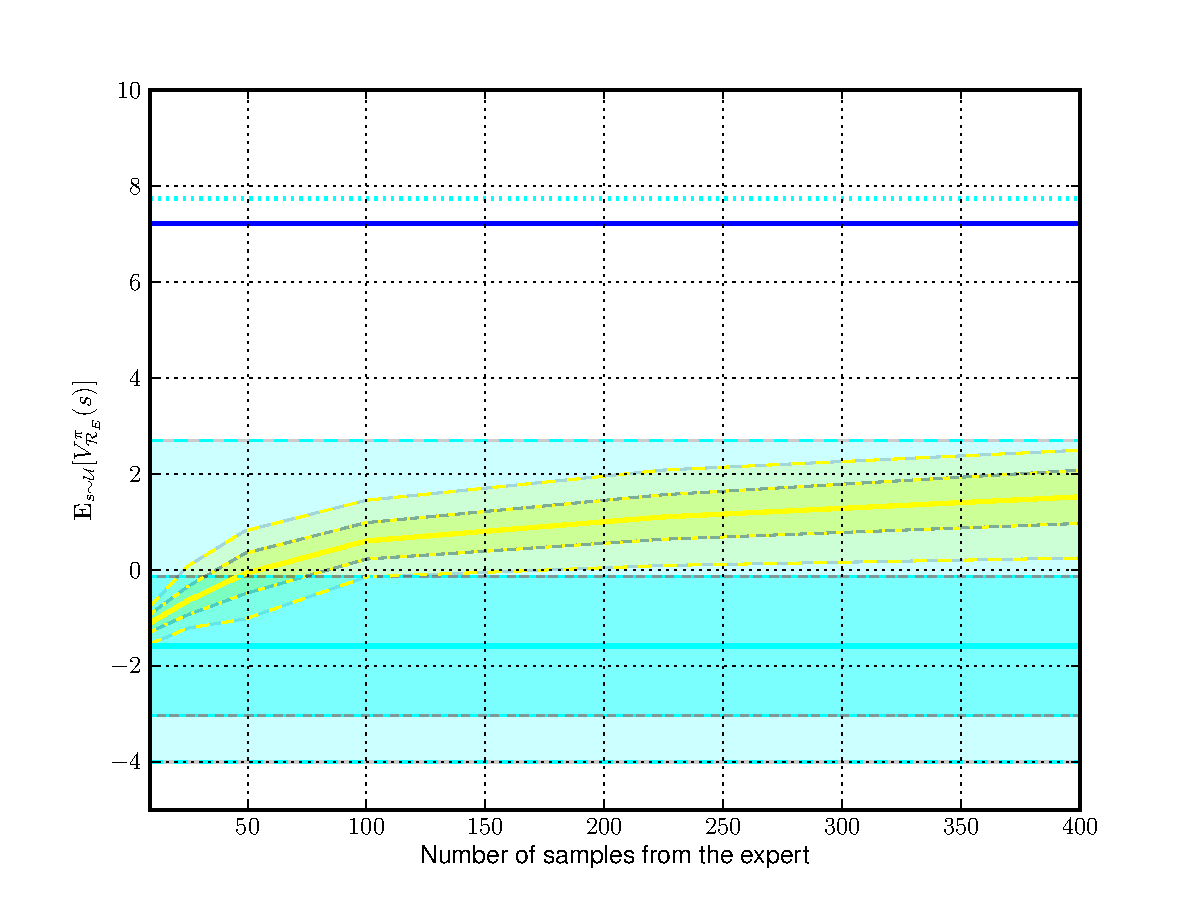
\includegraphics[width=.92\linewidth]{fig_classif.pdf}}
\end{minipage} \hfill
\begin{minipage}[r]{0.5\linewidth}
\centering
  \centerline{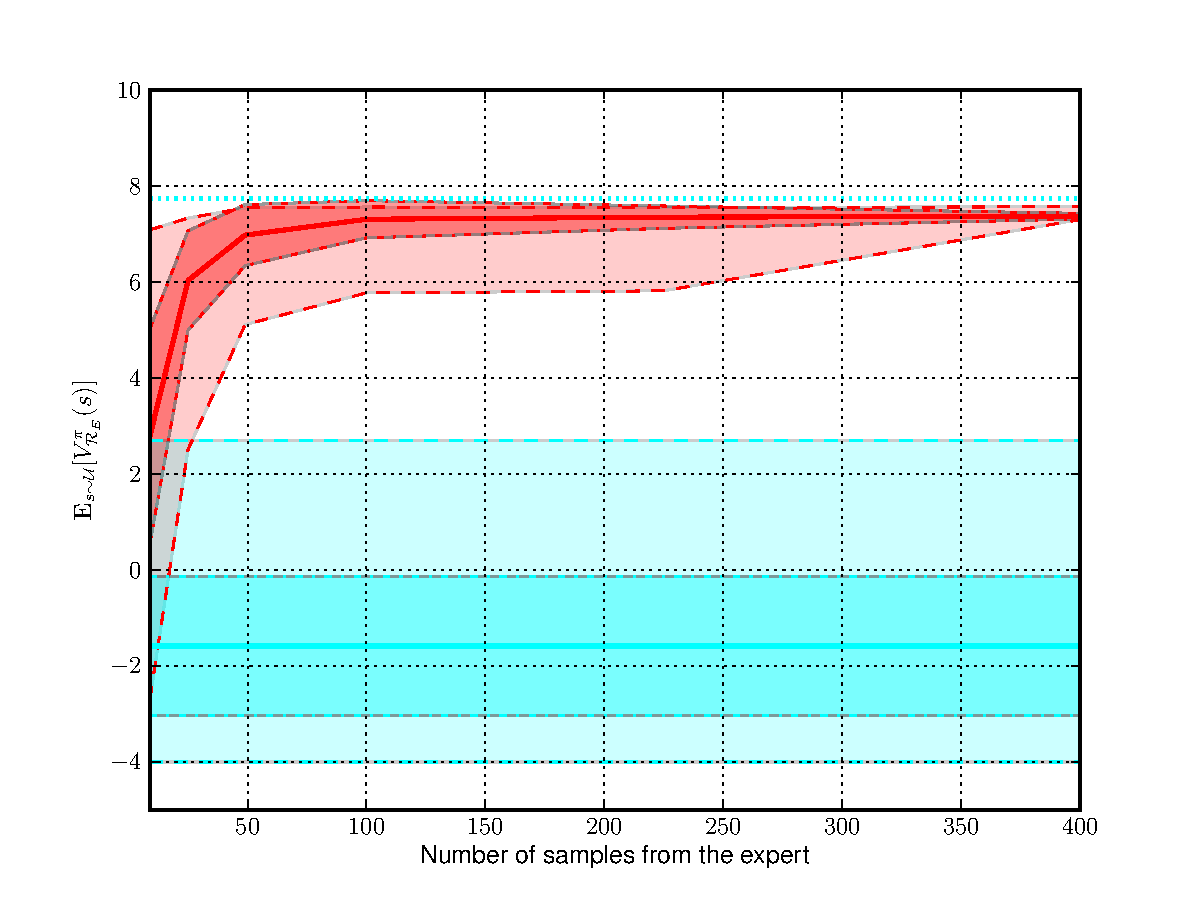
\includegraphics[width=.92\linewidth]{fig_scirl.pdf}}
\end{minipage}
  \caption{Highway problem. The highest line is the expert value. For each curves,
  we show the mean (plain line), the standard deviation (dark color) and the min-max values (light color).
  The policy corresponding to the random reward is in blue, the policy outputted by the  classifier is
  in yellow and the optimal policy according the SCIRL's reward is in red. PIRL is the dark blue line.}
  \label{fig:res}
\end{figure}

Fig.~\ref{fig:res} shows the performance of each approach as a
number of used expert transitions (except PIRL which uses the
model). We can see that the classifier does not work well on this
example. Increasing the number of samples would improve its
performance, but after 400 transitions it does not work as well as
SCIRL with only a ten of transitions. SCIRL works pretty well here:
after only a hundred of transitions it reaches the performance of
PIRL, both being close to the expert value. We do not report exact
computational times, but running SCIRL one time with $400$
transitions is approximately hundred time faster than running PIRL
for $70$ iteration.
%
% (this is due to the need to repeatedly solve MDPs for PIRL).

%Recall that for SCIRL the instantiation of
%Sec.~\ref{subsec:practicalApproach:instantiation} is considered,
%with a single Monte-Carlo rollout for estimating
%$\hat{\mu}^{\pi_E}(s_i,a_i)$ and using the proposed heuristic for
%$\hat{\mu}^{\pi_E}(s_i,a\neq a_i)$, which goes beyond our analysis.
%To our knowledge, it is the only algorithm working (at least on this
%benchmark) only with data from the expert.


\section{Conclusion}
\label{sec:conclusion}

We have introduced a new way to perform IRL by structuring a
linearly parameterized score function-based multi-class
classification algorithm with an estimate of the expert feature
expectation. This outputs a reward function for which we have shown
the expert to be near optimal, provided a small classification error
and a good expert feature expectation estimate. How to practically
estimate this quantity has been  discussed and we have introduced a
heuristic for the case where only transitions from the expert are
available, along with a specific instantiation of the SCIRL
algorithm. We have shown on a car driving simulator benchmark that
the proposed approach works well (even combined with the introduced
heuristic), much better than the unstructured classifier and as well
as a state-of-the-art algorithm making use of the model (and with a
much lower computational time). In the future, we plan to deepen the
theoretical properties of SCIRL (notably regarding possible
heuristics) and to apply it to real-world robotic problems.

\paragraph*{Acknowledgments.}

This research was partly funded by the EU FP7 project ILHAIRE (grant
n�270780), by the EU INTERREG IVa project ALLEGRO and by the R�gion
Lorraine (France).

\newpage
%\small
\bibliographystyle{plain}%{unsrt}
\bibliography{scirl_nips}
\end{document}
